\documentclass[a4paper,12pt]{article}
\usepackage{amsmath,amsthm,amsfonts,amssymb,amscd,amstext,vmargin,graphics,graphicx,tabularx,multicol} 
\usepackage[francais]{babel}
\usepackage[utf8]{inputenc}  
\usepackage[T1]{fontenc} 
\usepackage{pstricks-add,tikz,tkz-tab,variations}
\usepackage[autolanguage,np]{numprint} 


\setmarginsrb{2.5cm}{0.5cm}{2cm}{2cm}{0cm}{0cm}{0cm}{0cm} %Gauche, haut, droite, haut
\newcounter{numexo}
\newcommand{\exo}[1]{\stepcounter{numexo}\noindent{\bf Exercice~\thenumexo} : \marginpar{\hfill /#1}}
\reversemarginpar


\newcounter{enumtabi}
\newcounter{enumtaba}
\newcommand{\q}{\textbf{\stepcounter{enumtabi} \theenumtabi)}  }
\newcommand{\qa}{\textbf{\stepcounter{enumtaba} (\alph{enumtaba})} }
\newcommand{\initq}{\setcounter{enumtabi}{0}}
\newcommand{\initqa}{\setcounter{enumtaba}{0}}

\newcommand{\be}{\begin{enumerate}}
\newcommand{\ee}{\end{enumerate}}
\newcommand{\bi}{\begin{itemize}}
\newcommand{\ei}{\end{itemize}}
\newcommand{\bp}{\begin{pspicture*}}
\newcommand{\ep}{\end{pspicture*}}
\newcommand{\bt}{\begin{tabular}}
\newcommand{\et}{\end{tabular}}
\renewcommand{\tabularxcolumn}[1]{>{\centering}m{#1}} %(colonne m{} centrée, au lieu de p par défault) 
\newcommand{\tnl}{\tabularnewline}

\newcommand{\bmul}[1]{\begin{multicols}{#1}}
\newcommand{\emul}{\end{multicols}}

\newcommand{\trait}{\noindent \rule{\linewidth}{0.2mm}}
\newcommand{\hs}[1]{\hspace{#1}}
\newcommand{\vs}[1]{\vspace{#1}}

\newcommand{\N}{\mathbb{N}}
\newcommand{\Z}{\mathbb{Z}}
\newcommand{\R}{\mathbb{R}}
\newcommand{\C}{\mathbb{C}}
\newcommand{\Dcal}{\mathcal{D}}
\newcommand{\Ccal}{\mathcal{C}}
\newcommand{\mc}{\mathcal}

\newcommand{\vect}[1]{\overrightarrow{#1}}
\newcommand{\ds}{\displaystyle}
\newcommand{\eq}{\quad \Leftrightarrow \quad}
\newcommand{\vecti}{\vec{\imath}}
\newcommand{\vectj}{\vec{\jmath}}
\newcommand{\Oij}{(O;\vec{\imath}, \vec{\jmath})}
\newcommand{\OIJ}{(O;I,J)}


\newcommand{\reponse}[1][1]{%
\multido{}{#1}{\makebox[\linewidth]{\rule[0pt]{0pt}{20pt}\dotfill}
}}

\newcommand{\titre}[5] 
% #1: titre #2: haut gauche #3: bas gauche #4: haut droite #5: bas droite
{
\noindent #2 \hfill #4 \\
#3 \hfill #5

\vspace{-1.6cm}

\begin{center}\rule{6cm}{0.5mm}\end{center}
\vspace{0.2cm}
\begin{center}{\large{\textbf{#1}}}\end{center}
\begin{center}\rule{6cm}{0.5mm}\end{center}
}


\begin{document}
\pagestyle{empty}
\titre{Contrôle : Les limites de fonctions}{Nom :}{Prénom :}{\textbf{TCOM}}{Date:}

\vspace*{0.25cm}

\exo{4} \textit{Conjecturer une limite}
\bmul{2}
\includegraphics[scale=1.25]{limite.eps} 

\columnbreak


\color{purple}
Graphiquement, on trouve :\\

$\lim\limits_{x \rightarrow -\infty} f(x)= 0$ et $\lim\limits_{x \rightarrow +\infty} f(x)= 0$\\
La courbe admet une asymptote horizontale d'équation y = 0 en $+\infty$ et en $-\infty$.\\

$\lim\limits_{\substack{x \rightarrow -1 \\ x<-1}} f(x) = + \infty$ et $\lim\limits_{\substack{x \rightarrow -1 \\ x>-1}} f(x) = - \infty$\\
La courbe admet une asymptote verticale d'équation $x=-1$.\\

\color{purple}
$\lim\limits_{\substack{x \rightarrow 1 \\ x<1}} f(x) = -\infty$ et $\lim\limits_{\substack{x \rightarrow 1 \\ x>1}} f(x) = + \infty$\\
La courbe admet une asymptote verticale d'équation $x=1$.

\color{black}





\emul



\exo{7} \textit{Calculs de limites}



\initqa \qa $\lim\limits_{\substack{x \rightarrow +\infty}} \left( x-10+e^x \right)$\\


\color{purple}

On a : $\lim\limits_{x \rightarrow +\infty} x-10= +\infty$ et 
   $\lim\limits_{x \rightarrow +\infty}e^x= +\infty$  \\
  
\textbf{ Par somme,} $\lim\limits_{x \rightarrow + \infty} \left( x-10+e^x \right) = +\infty$ \\


\color{black}


\qa $\lim\limits_{\substack{x \rightarrow -\infty}} \left( x-10+e^x\right) $\\


\color{purple}

On a : $\lim\limits_{x \rightarrow -\infty} x-10= -\infty$ et 
   $\lim\limits_{x \rightarrow -\infty}e^x= 0$  \\
  
\textbf{ Par somme,} $\lim\limits_{x \rightarrow -\infty} \left( x-10+e^x \right) = -\infty$ \\


\color{black}






\qa $\lim\limits_{\substack{x \rightarrow 3 \\ x>3}} \left( \dfrac{2x-1}{3-x} \right)$\\

\color{purple}
Etude du signe de $3-x$: \hspace*{1cm} $3-x>0$ $\Leftrightarrow$ $-x>-3$ $\Leftrightarrow$ $x<3$\\

On a : $\lim\limits_{\substack{x \rightarrow 3 \\ x>3}} 2x-1 = 5 $ et 
   $\lim\limits_{\substack{x \rightarrow 3 \\ x>3}} 3-x = 0^- $ \\
  
\textbf{ Par quotient,} $\lim\limits_{\substack{x \rightarrow 3 \\ x>3}} \left( \dfrac{2x-1}{3-x} \right)=-\infty$\\


\color{black}



\qa  $\lim\limits_{\substack{x \rightarrow 0 \\ x>0}}\left( \dfrac{3x^3-7}{1-e^x}\right) $\\


\color{purple}
Etude du signe de $1-e^x$: \hspace*{1cm} $1-e^x>0$ $\Leftrightarrow$ $-e^x>-1$ $\Leftrightarrow$ $e^x<1$ $\Leftrightarrow$ $e^x<e^0$ $\Leftrightarrow$ $x<0$\\

On a : $\lim\limits_{\substack{x \rightarrow 0 \\ x>0}} 3x^3-7  = -7 $ et 
   $\lim\limits_{\substack{x \rightarrow 0 \\ x>0}} 1-e^x = 0^- $ \\
  
\textbf{ Par quotient,}  $\lim\limits_{\substack{x \rightarrow 0 \\ x>0}}\left( \dfrac{3x^3-7}{1-e^x}\right)=+\infty $\\


\color{black}



\qa  $\lim\limits_{\substack{x \rightarrow +\infty }} \left( \dfrac{1}{2x\sqrt{x}}-5\right) $\\


\color{purple}


On a :  $\lim\limits_{\substack{x \rightarrow +\infty }} 2x =+\infty$ et 
  $\lim\limits_{\substack{x \rightarrow +\infty }} \sqrt{x} =+\infty$ \\
  
\textbf{ Par produit,}  $\lim\limits_{\substack{x \rightarrow +\infty }} 2x\sqrt{x} =+\infty$\\

\textbf{ Par quotient,}  $\lim\limits_{\substack{x \rightarrow +\infty }} \dfrac{1}{2x\sqrt{x}} =0$\\

\textbf{ Par somme,}  $\lim\limits_{\substack{x \rightarrow +\infty }} \left( \dfrac{1}{2x\sqrt{x}}-5\right)=-5 $\\




\color{black}



\exo{3.5} Soit $f$ la fonction définie sur $\R \backslash \left\lbrace -2 \right\rbrace$ dont le tableau de variation est le suivant :\\

\begin{variations}
x          & \mI &       &  & -2& &  & 2& & \pI \\
\filet
$\m{f}$ &  3   &   \c & \h\pI & \bb & \mI & \c & \h1 & \d &0 \\
\end{variations}

\vspace*{0.25cm}

\noindent \initqa \qa Donner toutes les limites de $f$ qui sont renseignées dans ce tableau.\\

\color{purple}

D'après le tableau de variation, on a : \\
$\lim\limits_{x \rightarrow -\infty} f(x)=3$ ; \hspace*{0.5cm}    $\lim\limits_{x \rightarrow -2^-} f(x)=+\infty$ ; \hspace*{0.5cm}    $\lim\limits_{x \rightarrow -2^+} f(x)=-\infty$  ; \hspace*{0.5cm}    $\lim\limits_{x \rightarrow +\infty} f(x)=0$ \\
  

\color{black}


\qa Dans un repère, $C_f$ est la courbe représentative de $f$.\\
 Déterminer les asymptotes de $C_f$.\\
 
 \color{purple}

La courbe $C_f$ admet une asymptote verticale d'équation $x=-2$, une asymptote horizontale d'équation $y=3$ et une asymptote horizontale d'équation $y=0$.\\
  

\color{black}

\qa Montrer que l'équation $f(x)=0$ admet une unique solution sur $\R$.\\

\color{purple}

\bi
\item \textbf{Dans l'intervalle $]-\infty;-2[$:}\\
On a $f(x)>3$.\\
Donc l'équation $f(x) = 0$ ne possède pas de solution sur $]-\infty;-2[$.\\

\item \textbf{Dans l'intervalle $]-2;2[$:}\\
 D'après le tableau de variations, la fonction $f$ est continue et strictement croissante sur $]-2;2[$.\\
On a  $\lim\limits_{x \rightarrow -2^+} f(x)= -\infty$ et f(2)=1.\\
Or, $0 \in ]-\infty ; 1[$\\
Donc d'après le cas particulier du théorème des valeurs intermédiaires, l'équation $f (x) = 0$ admet une unique solution dans $]-2;2[$.\\

\item \textbf{Dans l'intervalle $]2;+\infty[$:}\\
On a   f(2)=1 et $\lim\limits_{x \rightarrow +\infty} f(x)=0$ .\\
Or, $0 \in ]1;0[$\\
Donc l'équation $f(x) = 0$ ne possède pas de solution sur $]2;+\infty[$.\\

\item On déduit de cette étude que l'équation $f(x)=0$ possède une unique solution sur $\R$.\\
\ei
  

\color{black}


\exo{5.5}\\


\begin{variations}
x          & \mI &      &       & -2   &     &  &  &     &   1&   &    & \pI \\
\filet
$\m{f   }$ &  2  &   \c & \h\pI & \bb & \mI &  & \c &  \h\pI & \bb & \mI & \c & \h1 \\
\end{variations}

\vspace*{0.5cm}

\noindent \initq \q Justifier la continuité de la fonction $f$.\\
\color{purple}
D'après la lecture du tableau de variations, la fonction $f$ est continue sur $]-\infty;-2[$ puis sur  $]-2;1[$ puis sur  $]1;+\infty[$.\\
\color{black}




\q Déterminer le nombre de solutions de $f(x)=0$ sur  $\R$.\\

\color{purple}

\bi
\item \textbf{Dans l'intervalle $]-\infty;-2[$:}\\
On a $f(x)>2$.\\
Donc l'équation $f(x) = 0$ ne possède pas de solution sur $]-\infty;-2[$.\\

\item \textbf{Dans l'intervalle $]-2;1[$:}\\
 D'après le tableau de variations, la fonction $f$ est continue et strictement croissante sur $]-2;1[$.\\
On a  $\lim\limits_{x \rightarrow -2^+} f(x)= -\infty$ et $\lim\limits_{x \rightarrow 1^-} f(x)= +\infty$.\\
Or, $0 \in ]-\infty ; +\infty[$\\
Donc d'après le cas particulier du théorème des valeurs intermédiaires, l'équation $f (x) = 0$ admet une unique solution dans $]-2;1[$.\\

\item \textbf{Dans l'intervalle $]1;+\infty[$:}\\
D'après le tableau de variations, la fonction $f$ est continue et strictement croissante sur $]1;+\infty[$.\\
On a  $\lim\limits_{x \rightarrow 1^+} f(x)= -\infty$ et $\lim\limits_{x \rightarrow 1^+} f(x)= 1$.\\
Or, $0 \in ]-\infty ; 1[$\\
Donc d'après le cas particulier du théorème des valeurs intermédiaires, l'équation $f (x) = 0$ admet une unique solution dans $]1;+\infty[$.\\

\item On déduit de cette étude que l'équation $f(x)=0$ possède deux solutions sur $\R$.\\
\ei
  

\color{black}


\q \textbf{BONUS :} Déterminer la valeur des solutions $\alpha_1$ et $\alpha_2$. En déduire le signe de $f(x)$ en fonction des valeurs de $x$.\\

\color{purple}
Tableau de signe :\\

\begin{variations}
 x      & \mI &  & -2 & & $\alpha_1$   &  &1&  &     &  &$\alpha_2$ &  & +\infty \\
\filet
f'(x) & \ga+     & \bb  & -&      \z     & +&\bb &   &  - &  & \z       & +     \\
\end{variations}


\end{document}
